\subsection{Authorization flows}
This section describes the two authorization flows in the OAuth specification, the authorization code grant and the implicit grant.
Due to the weaker security properties of the implicit grant, the authorization code grant should be preferred over the implicit grant where possible.
As such, the main focus of this section is on the authorization code grant.

\subsubsection{Authorization code grant}
\label{sec:background-oauth-code}

The OAuth specification defines an authorization code grant, which can be used to obtain access tokens and refresh existing tokens.  
The authorization flow is based on redirections.  Parameters are passed as query parameters to the authorization server using the \textit{application/x-www-form-urlencoded} format \citep{noauthor_post_2023}.
A typical authorization code grant, described in figure \ref{oauth_code_flow}, functions as follows
\citep{hardt_oauth_2012}:
\begin{enumerate}
    \item \textbf{Initiate authorization} \\
    The resource owner, or end user, initiates the authorization process.
    This could be a user clicking a login button, a user trying to perform an action requiring authorization or a user wanting to give access to some of its information to a third party.
    \item \textbf{Redirect end user to authorization endpoint} \\
    The client handles the authorization request by directing the resource owner to the authorization server.
    The client passes the client identifier, the requested scope and can optionally pass the local state to the authorization server.
    The state is an opaque value, such as a hash of a unique user session identifier, that is used by the client to maintain state between the request and the callback.
    State is used to protect clients against Cross-site request forgery (CSRF) attacks, where the user-agent of a victim is made to follow a malicious URI to a trusting server, allowing attackers to inject their own authorization code to the request, which can cause victims to be signed in as the attacker or can even give the attackers access to protected resources belonging to the victim. 
    A redirection URI is also included, to which the authorization server should redirect the end user to once the authorization process is complete.
    \item \textbf{Authenticate user} \\
    The authorization server authenticates the end user.
    The OAuth specification does not define how this authentication is implemented, leaving it up to each authorization server.
    Typical authentication methods are traditional username and password or biometrics and can include multi-factor authentication methods (MFA).
    The authorization server requires the end user to confirm the authorization to the specific client, preventing common CSRF attacks.
    \item \textbf{Authorization response} \\
    If the end user grants access and is successfully authenticated, the authorization server responds with an authorization response.
    The response contains an authorization code and the client state, if it was passed in the initial authorization request.
    The response is sent to the redirect URI that was sent in the authorization request.
    \item \textbf{Request access token} \\
    After obtaining an authorization code, the client requests an access token from the authorization server.
    The request includes the authorization code, in addition to a client identifier and redirect URI.
    The request can also include a scope for the token, which the authorization server takes into account when generating the token, limiting what the token can be used for.
    \item \textbf{Access token response} \\
    The authorization server confirms that the authorization code is valid and authorized, and ensures that the code was issued to the client that is making the token request. 
    After validating the code, the server responds with an access token, an expiration time and an optional refresh token.
    The scope of the access token should be the same as requested in the token request, if a scope was included.
    The authorization server takes the client identity into account when deciding the token scope, making it possible for the token to be given less rights than was requested.
    \item \textbf{Request protected resource} \\
    The client can now use the access token to access protected resources by adding the token to the request body, to the request headers or as a query parameter, depending on the resource server.
    This request can be repeated by the client as long as the access token is still valid.
    \item \textbf{Introspection request} \\
    When receiving a request for a protected resource, the resource server has to validate the provided access token.
    How this token validation should be implemented is not defined in the original OAuth 2.0 specification, but it is defined in a separate OAuth 2.0 Token Introspection specification \citep{richer_oauth_2015}.
    The only required parameter for the token introspection request is the access token itself, with the option to send additional parameters, such as a token type hint.
    \item \textbf{Introspection response} \\
    The authorization server responds with a JSON object containing information about the token, with a boolean value indicating if the token is active as well as a unique identifier, \textit{sub}, as the only required parameters.
    The response can also contain a number of parameters describing the token, such as an identifier for the client it was issued, the username of the resource owner, the scope of the token or the token type.
    The response can also include an expiry time, a timestamp for when the token was originally issued, a timestamp for when the token becomes active, a subject for the token, the intended audience for the token, the issuer of the token as well as a string identifier for the token.
    \item \textbf{Return the requested resource} \\
    Based on the parameters returned by the authorization server, the resource server can return the protected resource, perform an action requiring authorization or return some personalized data.
\end{enumerate}

\begin{figure}
	\centering
	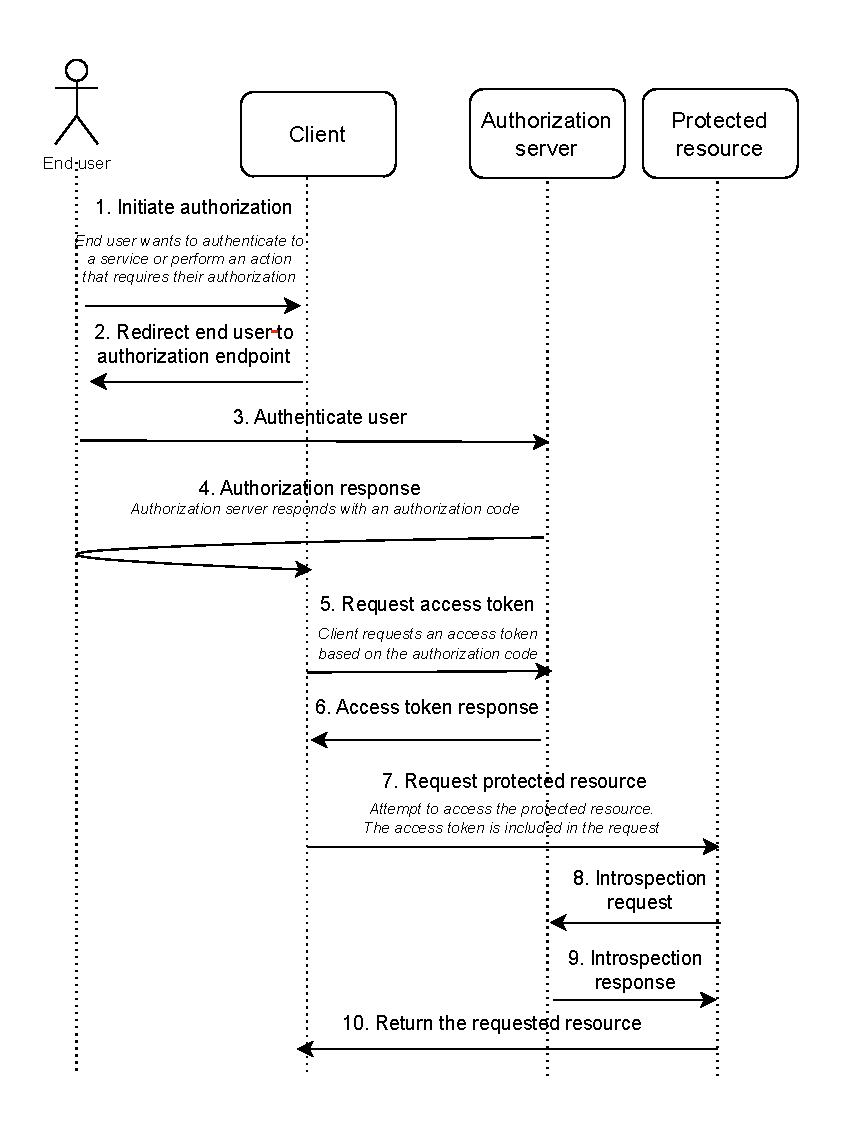
\includegraphics[height=190mm]{assets/oauth_authorization_code_grant.drawio.pdf}
	\caption{Accessing a protected resource using OAuth 2.0 authorization code grant.}
	\label{oauth_code_flow}
\end{figure}

\subsubsection{Implicit grant}
\label{sec:background-oauth-implicit}
Access tokens can also be obtained using the implicit grant type, which simplifies the authorization flow of the authorization code grant by removing the issuing of authorization codes.
This shortens the number of round-trips required, improving the responsiveness of interactive applications.
The steps of the implicit grant are similar to the authorization code grant described in figure \ref{oauth_code_flow}, with the authorization server responding with an access token directly, instead of issuing an authorization code first.
The implicit grant type removes the use of refresh tokens, requiring end users to authenticate multiple times if a session takes longer than the access token is valid.
As the access token is included in the response URI, there is an increased chance for the token leaking.
The implicit grant does not provide a method for identifying clients, making it impossible for authorization servers to validate that the used token was requested to the client using it.
